\section{Quadruple cut and box coefficients}\label{sect-quadcut}
The highest-point scalar integrals that can survive after reduction are the four-point ones, \ie boxes. 
Thus, the maxmial number of cut that can be done is four. 
Under a quadruple cut, bubble and triangle integrals vanish because they do not have enough propagators.
Hence, if we apply a quadruple cut on both sides of~\cref{master_equation}, we can identify the coefficients for the box integrals.
This process was proposed first by Britto, Cachazo and Feng~\cite{Britto:2004nc}.
\\\\
Analogous to the double cut case~\cref{cutkosky}, in the integrand of a quadruply cut generic amplitude, we will have four delta functions with positive energy and a product of four tree-level amplitudes, which are located at the ends of each cut. 
Therefore, under a quadruple cut,~\cref{master_equation} takes the form
\begin{equation*}
\int\dd^D l \delta^{(+)}(l^2) \delta^{(+)}\big((l-K_1)^2\big)\big((l-K_{12})^2\big)\big((l+K_4)^2\big)
A_1^{\mathrm{tree}}A_2^{\mathrm{tree}}A_3^{\mathrm{tree}}A_4^{\mathrm{tree}}=
\int_{i\in\mathrm{box}} c_i \Delta I_i
\end{equation*}
where $\Delta I_i$ are the cut box integrals.
\begin{figure}[h]
  \centering
  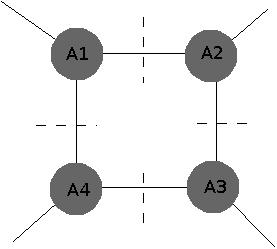
\includegraphics[width=0.5\linewidth]{quadruple_cut.jpg}
  \caption{Quadruple cut}
  \label{fig-quadruple_cut}
\end{figure}
The only box integral that survives such a quadruple cut should contain exactly the some propagators, which gives
\begin{equation}\label{quadcut_box}
\Delta I = \int \dd^D l \delta^{(+)}(l^2) \delta^{(+)}\big((l-K_1)^2\big)\big((l-K_{12})^2\big)\big((l+K_4)^2\big)
\end{equation}
We should note that the loop momentum $l$ should be treated as complex vector and the delta functions impose the integration contour on the complex plan~\cite{PhysRevD.75.025028, Kosower:2011ty}.
In generic cases, where all the external momenta $K_i$'s are not linear to each other, 
there are two solutions for $l$ under the constraint of the four delta functions in~\cref{quadcut_box}. 
Thus, the box coefficient $c$ is given by
\begin{equation}\label{box_coeff}
c = \frac{1}{2}\sum_{\mathcal{S}, J}n_J A_1^{\mathrm{tree}}A_2^{\mathrm{tree}}A_3^{\mathrm{tree}}A_4^{\mathrm{tree}}
\end{equation}
where $\mathcal{S}$ represents the set of solutions for the loop momentum $l$ under the contraint of the four delta functions in~\cref{quadcut_box} and $n_J$ is the number of intermediate particles having spin $J$.
\\\\
As an example, we will compute the all-gluon one-loop five-point MHV amplitude in $\mathcal{N} = 4$ super Yang-Mills $A_5^{\textrm{1-loop}}[g_1^- g_2^- g_3^+ g_4^+ g_5^+]$. 
In fact, by an argument of power counting using the background field method~\cite{Gates:1983nr} and the supersymmetric Ward identity\begin{equation}\label{super_wi}
\begin{split}
A^{\mathrm{tree}}(\Lambda_1^-, g_2^+, \ldots, g_j, \ldots, \Lambda_n^+)
= \frac{\langle jn \rangle}{\langle j 1 \rangle}
A^{\mathrm{tree}}(g_1^-, g_2^+, \ldots g_j^-, \ldots , g_n^+)
\\
A^{\mathrm{tree}}(\phi_1^-, g_2^+, \ldots, g_j, \ldots, \phi_n^+)
= \frac{\langle jn \rangle^2}{\langle j 1 \rangle^2}
A^{\mathrm{tree}}(g_1^-, g_2^+, \ldots g_j^-, \ldots , g_n^+)
\end{split}
\end{equation}
an $n$-point one-loop MHV amplitude in $\mathcal{\mathcal{N}} = 4$ can be written with only scalar box integrals~\cite{Bern:1994zx}.